%\necislovana{Seznam příloh}

\newpage
\part{Přílohy}
\label{prilohy}
\appendix

\newpage
%% ML: priloha bude jedna (zip), volil bych jednotne cislo
%% DT: zmeneno
\section{Struktura elektronické přílohy}
\label{ssec:struktura-příloh}

\setlength{\unitlength}{.5mm}
\begin{picture}(250, 220)
\put(  0, 212){\textbf{.}}
\put(  1, 200){\line(0, 1){5}}
\put(  1, 190){\line(0, 1){10}}
\put(  1, 190){\line(1, 0){10} {\textbf{ src}}}
\put( 16, 180){\line(0, 1){8}}
\put( 16, 180){\line(1, 0){10} {\textbf{ diff}}}
\put( 31, 170){\line(0, 1){8}}
\put( 31, 170){\line(1, 0){10} { klient.diff}}
\put(150, 170){Gisquick klient soubor diff}
\put( 31, 160){\line(0, 1){10}}
\put( 31, 160){\line(1, 0){10} { plugin.diff}}
\put(150, 160){Gisquick plugin soubor diff}
\put(  1, 140){\line(0, 1){50}}
\put(  1, 140){\line(1, 0){5} {\textbf{ text}}}
\put( 16, 130){\line(0, 1){8}}
\put( 16, 130){\line(1, 0){10} {\textbf{ LaTeX}}}
\put(150, 130){zdrojový kód programu LaTeX}
\put( 16, 120){\line(0, 1){10}}
\put( 16, 120){\line(1, 0){10} { david-tethal-dp-2018.pdf}}
\put(150, 120){text diplomové práce ve formátu PDF}
\put(  1, 100){\line(0, 1){50}} 
\put(  1, 100){\line(1, 0){10} {\textbf{ zadani}}} 
\put( 16, 90){\line(0, 1){8}}
\put( 16, 90){\line(1, 0){10} { zadanidp.pdf}} 
\put(150, 90){zadání diplomové práce}
\put(  1, 70){\line(0, 1){50}}
%% ML: v nazvu souboru/adresaru bych se vyvaroval diakritiky, klidne
%% nech anglicky nazev, jako je ted v gitu
%% DT: ponchan puvodni nazev
\put(  1, 70){\line(1, 0){10} {\textbf{ sample-project}}} 
\put(150, 70){vzorový QGIS projekt}

\end{picture}

\newpage
\section{Uživatelský manuál}
\label{uzivatelsky_manual}

Uživatelský manuál se skládá ze dvou částí. První obsahuje postup pro
instalaci a spuštění platformy Gisquick na lokálním zařízení. Druhá
%% ML: obsahuje popis / popisuje?
%% DT: popis
část obsahuje popis uživatelského rozhraní zásuvného modulu pro platformu QGIS
a dále Gisquick webového klienta. Uživatelský manuál je vytvořen
pouze pro části, které obsahují rozhraní pro práci s časoprostorovými
%% ML: lokalizovano v anglickem jazyce a take text uzivatelskeho
%% manual je napsan v anglickem jazyce
daty. Vzhledem k mezinárodnímu použití platformy Gisquick je text
uživatelského rozhraní, stejně jako instalační manuál, napsán 
v anglickém jazyce.

\subsection{Instalace}
\label{sssec:manual-instalace}

Zatímco pro webový server je vytvořen Docker kontejner a je tedy možné spustit jej pomocí Docker aplikace. Webový klient vyžaduje odlišný přístup zahrnující instalaci externích knihoven.

\bigskip
\noindent
\textbf{Webový server}

\noindent
Pro spuštění webového serveru na lokálním zařízení je nutná instalace Docker aplikace. Konfigurační soubor pro webový server \textit{docker-compose-dev.yml} se nachází ve složce ./docker větve vue-client v repozitáři dp-tethal-2018-gisquick \newline \url{https://github.com/ctu-geoforall-lab-projects/dp-tethal-2018-gisquick/tree/vue-client/docker}.
Před samotným spuštěním kontejneru je nejprve nutné vytvořit adresářovou strukturu, obsahující publikovaný projekt.
Příkazem \newline \verb|$ mkdir -p _data/publish _data/media _data/data | \newline \verb|_data/etc/letsencrypt/live| \cite{gisquick-manual}. 

\noindent
Složku s publikovaným projektem je dále nutné nahrát do složky ./docker/\textunderscore data/publish. Dále je možné spustit samotný Docker kontejner ze složky ./docker
příkazem \newline \verb|docker-compose -f docker-compose-dev.yml up|

\noindent
Pro vytvoření nového uživatele je nutné postupovat podle kroků popsaných v oficiální dokumentaci platformy Gisquick \url{http://gisquick.readthedocs.io/en/latest/administrator-manual/user-management.html}

\bigskip
\noindent
\textbf{Webový klient}

\noindent
Pro spuštění webového serveru na lokálním zařízení je nutná instalace aplikace Node.js minimální verze 4.0.0 a dále manažer knihoven npm minimální verze 3.0.0. Ve složce ./clients/vue-js je nutné spustit příkaz \newline \verb|npm install| \newline který nainstaluje všechny nutné externí knihovny a pro samotné spuštění klienta příkaz \newline \verb|npm run dev| \newline který spustí aplikaci na URL \verb|http://localhost:8080|


\newpage
\subsection{Grafické uživatelské rozhraní}
\label{sssec:manual-gui}

Time support for Gisquick platform allows users to easily filter 
map content based on its spatio-temporal value. Any vector layer that 
contain attribute with time value may be used. 

This section contains user manual describing process of time layers 
publication in Gisquick plugin for QGIS together with functions of time
%% ML: client
filtering tool in Gisquick client.  

\bigskip
\noindent \textbf{Publication process}

%% ML: small settings, prepsat
%% DT: simple
There is simple settings in order to keep publication process easy to 
handle for any user. Time layer may be set up in the first
page of the publication wizard in the tab \textit{Layers}.  Dropdown
menu \textbf{Time Attribute} defines which layer attribute contains
%% ML: In case that ? nebo lepe...
%% DT: in cae that
time values. In case that this column is left blank, layer won't be listed
in the time filter tool. Second option is \textbf{Date Mask}. Time
values may have different formats in different countries. No matter
how original time format looks like, date mask offers a possibility to
customize displayed date format in Gisquick client.

\begin{figure}[h!]
	\centering
	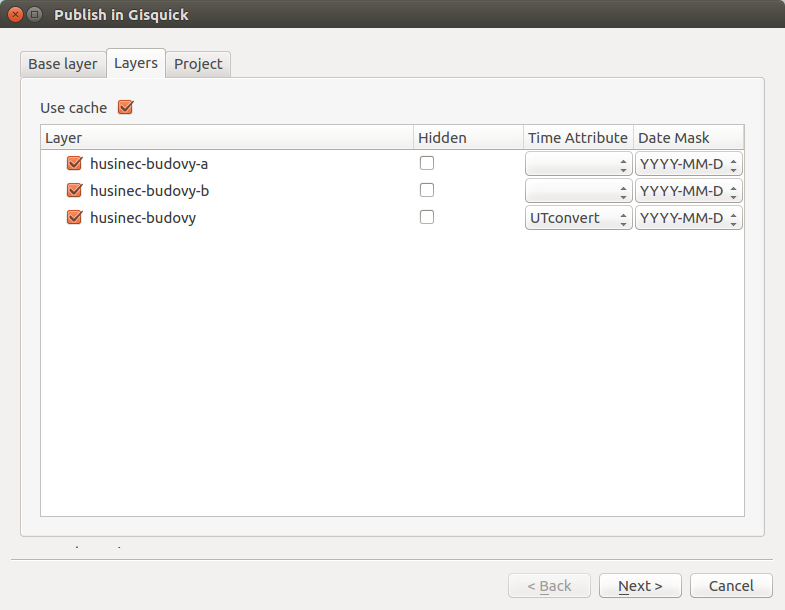
\includegraphics[width=0.75\textwidth]{../img/plugin-layers.png}
	\caption{Time layers options in publication wizard}
	\label{fig:publication-wizard-layers}
\end{figure}

Every user should know how the data looks like. 
\textbf{Date Mask} changes user interface of the time filtering tool. 
E.g. if 'HH:mm' mask is selected date picker will not be 
displayed in the client side, only time picker. 

It is recommended to use time date in format starting with 
year or hour excluding special character e.g. 'YYYY-MM-DD' or 'HH-mm'. 
Otherwise, new attribute containing time values in UNIX time format 
has to be created during publication process.

The \textbf{configuration summary} wizard page displays all the parameters 
that were computed for each time layer. Note that if the 
\textbf{Time Attribute} field was left blank, parameters will not have any 
value.

\begin{figure}[h!]
	\centering
	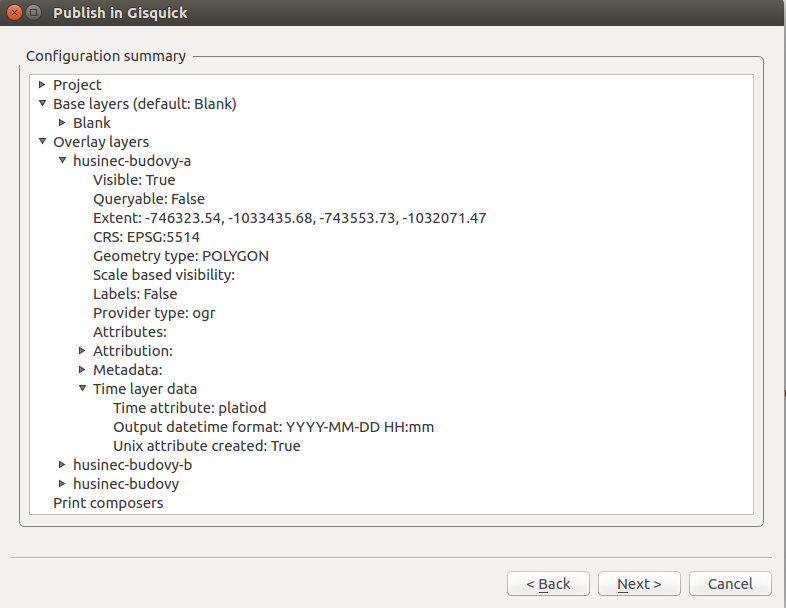
\includegraphics[width=0.7\textwidth]{../img/project-publishing-time-summary.png}
	\caption{Time layers publication summary}
	\label{fig:publication-wizard-summary}
\end{figure}

\bigskip
\noindent \textbf{Time filtering tool}

Time filtering tool in Gisquick client is available in the tool menu 
in upper left corner. 

\begin{figure}[h!]
	\centering
	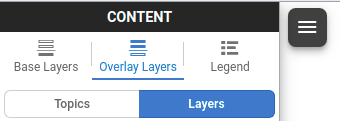
\includegraphics[width=0.4\textwidth]{../img/burger-menu.png}
	\caption{Tool menu}
	\label{fig:burger-menu}
\end{figure}

\bigskip
When the tool is activated dropdown menu with time layers appears on 
the left side of map canvas. For needs of filtration the time layer 
has to be specified. Despite selecting one time layer there is
also possibility of selecting \textit{All visible layers}.

\begin{figure}[h!]
	\centering
	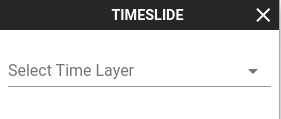
\includegraphics[width=0.4\textwidth]{../img/time-layers-dropdown.png}
	\caption{Dropdown menu containing time layers}
	\label{fig:time-layers-drpdown}
\end{figure}

\bigskip
It might happen that two time layers with different time extend are 
visible in the same time. E.g. one layer displaying map features 
over one hour and second over one year. Filtering this two layers 
together using one time slider would ignore layer with shorter time 
extend. That is the reason why only time layers with same time 
attribute may be displayed in the same time. In case `All visible 
layers` contains different time attribute. User have to specify one 
in displayed dropdown menu.

\begin{figure}[h!]
	\centering
	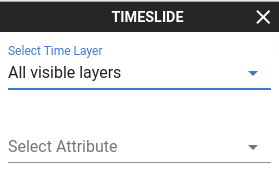
\includegraphics[width=0.4\textwidth]{../img/time-attribute-dropdown.png}
	\caption{Dropdown menu containing time attributes}
	\label{fig:time-attribute-dropdown}
\end{figure}

\newpage
Once filtering layer is specified various settings is displayed. 

\begin{figure}[h!]
	\centering
	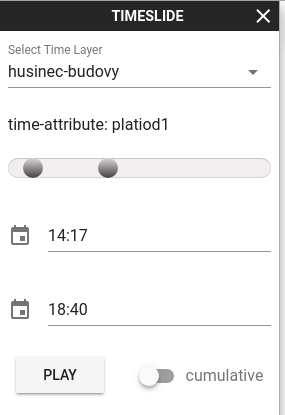
\includegraphics[width=0.4\textwidth]{../img/time-filtering-tool.png}
	\caption{Initialized time filtering tool}
	\label{fig:time-filtering-tool}
\end{figure}

Time filtering tool is composed of following parts:

\begin{itemize}
	\item\textit{Dropdown menu with time layers}
	\item\textit{Time attribute label}
	\item\textit{Double range slider}
	\item\textit{Lower and upper time value}
	\item\textit{Animation button with cumulative switch}
\end{itemize}

Function of \textbf{Dropdown menu with time layers} was mentioned before.
If selected time layer was already filtered, time filtering 
tool is initialized using previously used values.

\textbf{Time attribute label} displays name of attribute that was selected
in the process of project publishing as `Time Attribute`. This 
comes handy especially when `All visible layers` are selected.

\textbf{Double range slider} allows user to make fast data filtration.
Time interval is set using two sliders. Map content is refreshed 
each time the slider is changed. Step of double range slider is set 
as one hundredth of time interval size.

\begin{figure}[h!]
	\centering
	
\includegraphics[width=0.4\textwidth]{../img/time-slider.png}
	\caption{Double range slider}
	\label{fig:time-slider}
\end{figure}

Time interval may be specified with better precision than time 
slider using \textbf{Lower and upper time value} labels. Precision depends
on selected output time format in project publication. If format 
contains time and date, then labels allow user to set time using time
pickers and date in calendar. In case that time format contains date 
than is not more precise than one day, only calendar is displayed. 
Time and date 
selection in displayed date time picker has to be confirmed by 
\textit{OK} button. Map canvas is updated after this confirmation.

\begin{figure}[h!]
	\centering
	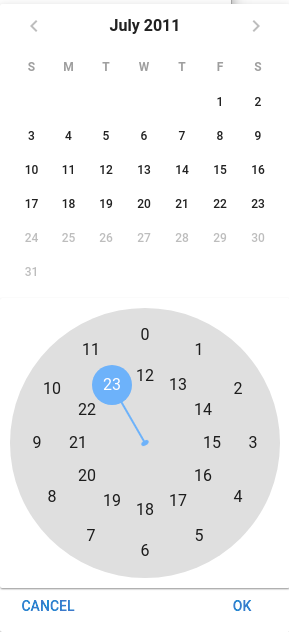
\includegraphics[width=0.3\textwidth]{../img/date-time-picker.png}
	\caption{Date time picker}
	\label{fig:date-time-picker}
\end{figure}

Simple animation can be made using \textbf{Animation button}. There are two 
options. Classic and cumulative animation. Classical one increases both 
upper and lower values every second by slider step. 
Animation stops when upper value reach slider maximum. If cumulative 
mode is turned on only upper value is being increased. When it reaches 
slider maximum than lower value increases in the same pattern.
Animation ends when difference between upper and lower value is just one 
step. Second  way how to stop animation may be click on \textit{STOP} button. 
Stop button appears only when animation is on. Map canvas is updated 
each time when slider value is changed.

\begin{figure}[h!]
	\centering
	
\includegraphics[width=0.4\textwidth]{../img/time-animation-stop.png}
	\caption{Time animation stop button}
	\label{fig:time-animation-stop}
\end{figure}

\newpage
\section{Seznam obrázků a tabulek}
\listoffigures
\listoftables


